%!TEX root = ../CombinatoricsNotes.tex

\section{Incidence problems}
\lect{4}{4}
% \marginnote{Lecture X: Monday, April 4, 2016.}
\begin{theorem}[Euler's formula]
Let $G$ be a connected graph drawn in the plane without crossings. Then
\[
|V(G)| - |\edges (G)| + \reg (G) =2
\]
where $\reg (G)$ is the number of regions in which the drawing divides the plane.
\end{theorem}

\begin{corollary} \label{cor:bound_edges_of_planar_3VG}
Let $G$ be a graph drawn in the plane without crossings. Then
\[
|\edges (G) |\leq 3 |V(G)|.
\]
\end{corollary}
\begin{proof}	
We assume $|V(G)|\geq 3$. By adding additional edges we can ensure that each region of the drawing has a cycle of length 3 as its boundary. Then
\[
3 \reg(G) = 2 |\edges (G)|
\]
by double counting pairs (edge, region) such that each edge belongs to two regions boundary. Substituting into Euler's formula, we have 
\[
|V(G)| - |\edges (G)| + \frac{2}{3}|\edges (G)| = 2
\]
so
\[
|\edges (G)| = 3 | V(G)| - 6 \leq 3 |V(G)|.
\]
\end{proof}

Let $\crossings(G)$ denote the minimal number of pairs of crossing edges taken over all drawing of $G$ in the plane  where vertices are represented by points, edges by curves joining corresponding points, and the drawing of edges are allowed to intersect, and each intersection is a \emph{crossing}\sidenote{locally looks like an $X$, not two curves bouncing off each other.}.

Then $\crossings(G)=0$ iff $G$ can be drawn in the plane without crossings, and $\crossings(K_5)=1$, by the drawing
\begin{center}
\begin{tikzpicture}

\end{tikzpicture}
\end{center}


\begin{corollary} \label{cor:bound_crossings_planar_graph93}
$\crossings(G) \geq |\edges (G)| - 3 |V(G)|$.
\end{corollary}
\begin{proof}	
Let $G$ be a graph with $\crossings(G) = c$. In a drawing of $G$ with $c$ pairs of crossing edges, remove $c$ edges to obtain a graph drawin without crossings. Then by \cref{cor:bound_edges_of_planar_3VG},
\[
|\edges (G)| - c \leq 3 |V(G)|
\]
as we wanted.
\end{proof}

\begin{theorem}[Crossing number lemma]
\label{thm:crossing_number_lemma}

\[
\crossings(G) \geq \frac{1}{64}\frac{m^3}{n^2}
\]
for every graph $G$ with $m$ edges and $n$ vertices such that $m\geq 4n$.
\end{theorem}
\begin{proof}	
Let $p \in [0,1]$ which we will choose later. Let $X\subset V(G)$ be obtained by choosing to include each vertex independently at random with probability $p$. Let $G'$ be the random subgraph of $G$ induced by $X$, namely $V(G') = X$, $\edges(G') = \edges(G| X)$. Let $m = |\edges(G)|$, $n= |V(G)|$, $x= \crossings(G)$, $m' = |\edges(G')|$, $n' = |V(G')|$, $x' = \crossings(G')$. Then by construction $\E[n'] = np$. Since each edge of $G$ survives with probability $p^2$, by linearity $\E[m']= mp^2$. Next, $\E[x'] \leq xp^4$ because the probability that a particular pair of crossing edges survives is $p^4$.

By \cref{cor:bound_crossings_planar_graph93}, $x'\geq m' - 3n'$. Taking expectation values, we have the bound $x p^4 \geq mp^2 - 3np$. That is,
\[
x\geq \frac{m}{p^2} - 3 \frac{n}{p^3}.
\]
Now, we choose optimal $p$:
\begin{gather*}
 \frac{\partial}{\partial p} \left( \frac{m}{p^2}- \frac{3n}{ p^3} \right) = - \frac{2m}{p^3} + \frac{9n}{p^4} = 0 \\
 \implies p=\frac{1}{4.5}\frac{n}{m}.
\end{gather*}
Let us simply take $p = \frac{1}{4}\frac{n}{m}.$ Then
\begin{gather*}
\crossings (G):=x \geq \frac{m}{\frac{16 n^2}{m^2}} - \frac{3n}{\frac{64 n^3}{m^3}}p = \frac{m^3}{n^2} \left( \frac{1}{16} - \frac{3}{64} \right) = \frac{1}{64}\frac{m^3}{n^2}.
\end{gather*}
\end{proof}

Let $P$ be a set of points in the plane. Let $L$ be a set of lines. Then define
\[
I(P,L):= |\{ ( p,L ): p\in P, l\in L, p\in L \}|.
\]
Then $I(P,L)$ is the number of \emph{incidences} of $P$ and $L$. Let $I(m,n)$ denote the maximum $I(P,L)$ over sets $P,L$ with $|P| = m$, $|L| = n$. Clearly, $I(m,n)\leq mn$.
\begin{example} We see $I(3,3) \leq 6$ by considering cases: if the three lines are parallel, the number of incidences is at most three. If two lines are parallel, there are at most five incidences. If none of the lines are parallel, there are at most six incidences. On the other hand, \cref{fig:I33} shows $I(3,3)\geq 6$.
\begin{marginfigure}
\begin{center}
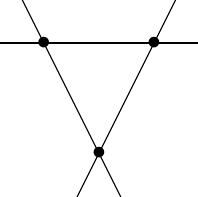
\begin{tikzpicture}[scale=.7,rotate=180]
\node (x) at (2,0) {$\bullet$};
\node (y) at (1,2) {$\bullet$};

\node (z) at (0,0) {$\bullet$};

% \node (w) at (1,0) {$w$};

\draw [shorten >=-1cm,shorten <=-1cm](x) -- (y);
\draw[shorten >=-1cm,shorten <=-1cm] (y) -- (z);
\draw[shorten >=-1cm,shorten <=-1cm] (z) -- (x);
\end{tikzpicture}
\vspace{1em}
\end{center}
\caption{We see $I(3,3)\geq 6$.} \label{fig:I33}
\end{marginfigure}
\end{example}




\begin{example}
Let $n=4k^3$. Set
\[
P = \{ (x,y): 0\leq x \leq k-1, 0 \leq y\leq 4k^2 - 1, x,y\in \Z\}
\]
and 
\[
L = \{ y = ax+b: 0\leq a \leq 2k-1, 0\leq b\leq 2k^2-1, a,b\in \Z \}
\]
Then $|P| = |L| =n$. We have $I(P,L)= k \cdot |L|  = kn \geq \frac{1}{2}n^{4/3}$

every line in $L$ incident with $k$ points in $P$.



\begin{gather*}
(x,ax+b)\in P \\
\text{for } 0\leq x \leq k-1, 0\leq a \leq 2k-1, 0\leq b \leq 2k^2- 1
\end{gather*}
$ax+b \leq (k-1)(2k-1) + 2k^2 - 1 < 4k^2$. So $I(n,n) \geq c n^{4/3}$ for all $n$ and some $c>0$.
\end{example}

\begin{theorem}[\cite{Szemeredi-Trotter1983}] \label{thm:bound_I_m_n95} \label{thm:Szemerdi_Trotter}
\[
I(m,n) \leq 4 m^{2/3} n^{2/3} + 4m + n.
\]
\end{theorem}

\begin{proof}	
Let $P,L$ be sets of points and lines such that $|P| = m$, $|L| = n$ and $I(P,L) = I(n,m)$. Let $G$ be a graph drawn in the plane with crossings such that $V(G)  = P$, and $\edges(G)$ are drawn as line segments joining consecutive points on lines in $L$. \marginnote{I.e., follow one line at a time, connecting consecutive points.}
Then
\[
\crossings(G)\leq n^2
\]
because every crossing in $G$ is an intersection of two lines in $L$ (loose estimate). Then
\[
I:=I(P,L) = |\edges(G)| + n
\]
if there is a point of $P$ on every line in $L$ (if not, delete that line). We see this by following each line in $L$, and noting between every two incidences, we have an edge: if there are $k$ points in $P$ on a single line, there are $k-1$ edges connecting them.

Then $|\edges(G)| = I -n$. We have $|\edges(G)|\leq 4 |V(G)|$ if $I - n \leq 4m$, that is $I\leq 4m + n$.

Otherwise,  by \cref{thm:crossing_number_lemma},
\[
n^2 \geq \crossings (G) \geq \frac{1}{64} \frac{|\edges(G)|^3}{|V(G)|^2} = \frac{1}{64} \frac{(I-n)^3}{m^2}.
\]
That is, 
\begin{gather*}
64 m^2 n^2 \geq (I-n)^3\\
4 m^{2/3} n^{2/3}\geq I- n\\
I \leq 4m^{2/3}n^{2/3}+n.\qedhere
\end{gather*}
\end{proof}

\begin{conjecture*}[\cite{Erdos-Szemeredi-1983}]
For every $\epsilon>0$ there exists $c_{\epsilon} > 0$ s.t. for every $A\subset \Z$,
\[
|A+A| + |A\cdot A| \geq c_{\epsilon} |A|^{2 - \epsilon},
\]
where $A+A = \{a+b: a,b\in A\}$ and $A\cdot A = \{a\cdot b: a,b\in A\}$.
\end{conjecture*}


\begin{theorem}[\cite{elekes1997number}] \label{thm:96_elekes}
There exists $c>0$ such that for every $A\subset \Z$, 
\[
|A+A|\cdot |A\cdot A| \geq c |A|^{5/2}.
\]
In particular, by the arithmetic-geometric inequality,
\[
|A+A| + |A\cdot A| \geq c |A|^{5/4}.
\]
\end{theorem}
\begin{proof}	
Let 
\[
 P = \{(a,b):a \in A+A, b\in A\cdot A\}.
 \] Then $|P| =|A+A|\cdot |A\cdot A| $.Choose
\[
L = \{y = a(x-b): a,b\in A\}.
\]
Then $|L| = |A|^2$. Next, 
\[
 I(P,L) \geq |A|^3
 \] since each line in $L$ contains $|A|$ points in $P$ as follows: $y = a(x-b)$, so choose $x= b+a' \in A+A$ for any $a' \in A$. Then $y = aa' \in A\cdot A$, so $(x,y) \in P$.

Therefore, by \cref{thm:bound_I_m_n95},
\begin{align*}	
|A|^3 &\leq I(P,L) \leq 4 |A|^{4/3} |A+A|^{2/3}|A\cdot A|^{2/3} + 4|A+A| \cdot |A\cdot A| + |A|^2.
\end{align*}
At least one of these three terms is $\frac{1}{3}$ of the LHS. Easy if it is not the first one. Otherwise: $\frac{1}{3}|A|^3 \leq 4 |A|^{4/3} |A+A|^{2/3} |A\cdot A|^{2/3}$, so
\[
\left(\frac{1}{12}\right)^{3/2}|A|^{5/2} \leq |A+A| \cdot |A\cdot A|. \qedhere
\]
\end{proof}